\documentclass[a4paper,preprint,11pt,authoryear]{elsarticle}
\usepackage[margin=2cm]{geometry}
\usepackage{amsmath,amsthm,longtable,float,multirow,parskip,bm,todonotes}
\usepackage[colorlinks=true, linkcolor=black, citecolor=black, urlcolor=black]{hyperref}

\DeclareMathOperator{\cov}{Cov}
\DeclareMathOperator{\Var}{Var}
\DeclareMathOperator{\vetor}{vec}
\DeclareMathOperator{\seno}{sin}
\DeclareMathOperator{\RMSSE}{RMSSE}
\DeclareMathOperator{\RMSE}{RMSE}
\DeclareMathOperator{\RelRMSE}{RelRMSE}
\DeclareMathOperator{\Base}{Base}
\DeclareMathOperator{\Rec}{Rec}
\DeclareMathOperator{\Uni}{Uni}
\newtheorem{proposition}{Proposition}
\newtheorem{corollary}{Corollary}
\allowdisplaybreaks
\sloppy
\widowpenalty=10000
\clubpenalty=10000

\journal{TBD}

\begin{document}

% In-text numbers generated by the targets pipeline
\IfFileExists{Tabelas/numbers.tex}{% Generated by the targets pipeline; do not edit.
\newcommand{\expOneReps}{1000}
\newcommand{\gainFtwoBrazilMax}{15.7}
\newcommand{\kappaFtwoBrazilMax}{0.59}
\newcommand{\gainFthreeSmallMax}{5.9}
\newcommand{\sepPenaltySmall}{2.9}
\newcommand{\sepPenaltyBrazil}{1.6}
\newcommand{\gainFthreeWeakBrazil}{0.5}
\newcommand{\gainFthreeWeakBrazilEst}{0.1}
\newcommand{\kappaNoiseSep}{0.12}
\newcommand{\expTwoIncohRange}{0.4--1.5}
\newcommand{\expTwoKappaRange}{0.65--0.97}
\newcommand{\expTwoGainRange}{0.5--2.4}
\newcommand{\expTwoSepVsBaseRange}{6--11}
\newcommand{\expTwoCtrlGainMax}{2.1}
\newcommand{\expTwoArimaSmallRange}{0.996--1.006}
\newcommand{\expTwoArimaLargeRange}{0.979--0.996}
\newcommand{\expTwoVarMaxDiff}{0.5}
\newcommand{\expTwoBlocksMaxDiff}{0.2}
\newcommand{\testSizeRange}{4.2--5.8}
\newcommand{\appTArima}{156}
\newcommand{\appKappaArima}{0.34}
\newcommand{\appGainArima}{2.0}
\newcommand{\appPArima}{0.020}
\newcommand{\appIncohArima}{17}
\newcommand{\appKappaVar}{0.60}
\newcommand{\appGainVar}{2.3}
\newcommand{\appIncohVar}{13}
\newcommand{\appKronArima}{0.07}
\newcommand{\appJointSepArimaRange}{0.986--1.019}
\newcommand{\appJointSepVarRange}{0.951--0.996}
\newcommand{\appJointSepEtsRange}{0.951--1.016}
\newcommand{\appNetJointSepStates}{5}
\newcommand{\appNetJointSepTotal}{15}
\newcommand{\appNetJointJointStates}{5}
\newcommand{\appNetJointJointTotal}{21}
\newcommand{\appNetJointJointRegions}{14}
\newcommand{\appNetJointSepRegions}{10}
\newcommand{\appNetPointTotal}{18}
\newcommand{\appNetPointRegions}{8}
\newcommand{\appNetPointStates}{1}
\newcommand{\appNetPlugTotal}{4.9}
\newcommand{\appNetPlugRegions}{4.5}
\newcommand{\appNetPlugStates}{3.2}
\newcommand{\appSepVsBaseStatesAdm}{1.6}
}{}

\begin{frontmatter}
  \title{Separability and the limits of multivariate forecast reconciliation}

  \author[label1,label2]{Ana Caroline Pinheiro} %% Author name
  \author[label1]{Rodrigo de Souza Bulhões}
  \author[label3]{Rob J. Hyndman}
  \author[label1,label4]{Paulo Canas Rodrigues}

  \affiliation[label1]{organization={Department of Statistics, Federal University of Bahia},
    city={Salvador},
    state={Bahia},
    country={Brazil}
  }
  \affiliation[label2]{organization={Secretary of Health of the State of Bahia},
    city={Salvador},
    state={Bahia},
    country={Brazil}
  }
  \affiliation[label3]{organization={Department of Econometrics \& Business Statistics, Monash University},
    city={Melbourne},
    state={Victoria},
    country={Australia}
  }

  \affiliation[label4]{organization={Department of Business Management, University of Pretoria},
    city={Pretoria},
    country={South Africa}
  }

  \begin{abstract}
    \todo[inline]{Abstract: write last, from tasks/revision-abstract-intro.md updated with results.}

  \end{abstract}

  \begin{keyword}
    Hierarchical time series \sep forecast reconciliation \sep minimum trace \sep separable covariance \sep employment forecasting
  \end{keyword}
\end{frontmatter}

\section{Introduction}
\label{sec:intro}

\todo[inline]{Introduction: adapt paragraphs 1--10 of tasks/revision-abstract-intro.md; write after results.}

% Section 2 draft: notation and reconciliation of several variables.

\section{Reconciling several variables}
\label{sec:setup}

\subsection{Notation}

We follow the notation of \citet{athanasopoulos2023forecast}, adapted to several variables. Suppose $m$ variables are each observed over the same hierarchy with $n$ series, of which $n_b$ are at the bottom level and $n_a = n - n_b$ are aggregates. For variable $j$, let $\bm{y}_{j,t}$ be the $n$-vector of all its series at time $t$, and $\bm{b}_{j,t}$ the $n_b$-vector of its bottom-level series. Then
\begin{equation}\label{eq:ysb}
  \bm{y}_{j,t} = \bm{S}\bm{b}_{j,t},
  \qquad
  \bm{S} = \begin{bmatrix}\bm{A}\\ \bm{I}_{n_b}\end{bmatrix},
\end{equation}
where the $(n_a \times n_b)$ matrix $\bm{A}$ gives the aggregation constraints. Equivalently, $\bm{C}\bm{y}_{j,t} = \bm{0}$ with $\bm{C} = [\bm{I}_{n_a}\ \ -\bm{A}]$, so that $\bm{C}\bm{S} = \bm{0}$. Figure~\ref{fig:HTS_M.ex} shows a three-level example with $n = 8$ and $n_b = 5$.

\begin{figure}[!htb]
  \centering
  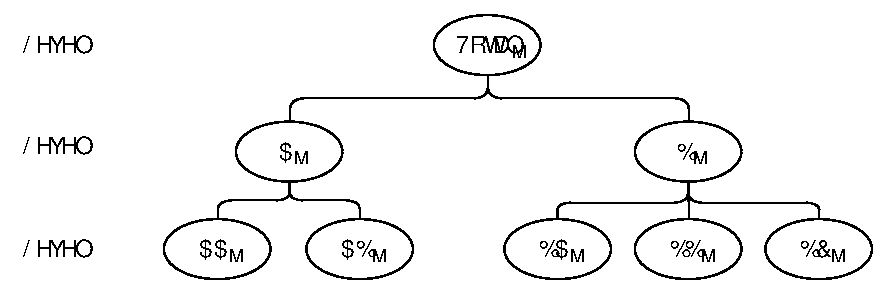
\includegraphics[width=11cm]{Imagens/diagrama_mult.pdf}
  \caption{A hierarchy with three levels, observed for each of $m$ variables.}
  \label{fig:HTS_M.ex}
\end{figure}

Collect the variables in $\bm{Y}_t = [\bm{y}_{1,t}, \dots, \bm{y}_{m,t}]$ and $\bm{B}_t = [\bm{b}_{1,t}, \dots, \bm{b}_{m,t}]$. Stacking the columns gives
\begin{equation}\label{eq:vec}
  \vetor(\bm{Y}_t) = \bm{S}_*\vetor(\bm{B}_t),
  \qquad
  \bm{S}_* = \bm{I}_m \otimes \bm{S},
\end{equation}
with constraint matrix $\bm{C}_* = \bm{I}_m \otimes \bm{C}$. The stacked summing matrix is block diagonal: no constraint links one variable to another. This distinguishes the setting from a grouped hierarchy, where the categories of a grouping variable (such as travel purpose in the Australian tourism data of \citealp{wickramasuriya2019optimal}) are linked by aggregation constraints because their total is itself observed and forecast.

\subsection{Forecast reconciliation}

Let $\widehat{\bm{y}}_{T+h|T}$ be the stacked $h$-step base forecasts of all $mn$ series, produced without regard to the constraints, and let $\bm{W}_h$ be the covariance matrix of their errors. Linear reconciliation maps the base forecasts to coherent forecasts $\widetilde{\bm{y}}_{T+h|T} = \bm{S}_*\bm{P}\widehat{\bm{y}}_{T+h|T}$ for some matrix $\bm{P}$ with $\bm{P}\bm{S}_* = \bm{I}$. The minimum trace (MinT) choice \citep{wickramasuriya2019optimal} minimises the trace of the reconciled error covariance and gives
\begin{equation}\label{eq:mint}
  \widetilde{\bm{y}}_{T+h|T} = \bm{S}_*(\bm{S}_*'\bm{W}_h^{-1}\bm{S}_*)^{-1}\bm{S}_*'\bm{W}_h^{-1}\widehat{\bm{y}}_{T+h|T}
  = \big[\bm{I} - \bm{W}_h\bm{C}_*'(\bm{C}_*\bm{W}_h\bm{C}_*')^{-1}\bm{C}_*\big]\widehat{\bm{y}}_{T+h|T},
\end{equation}
the second form being the zero-constrained representation of \citet{di2023cross}. Applied to the stacked system this is ordinary MinT with summing matrix $\bm{S}_*$; we call it \emph{joint} reconciliation. \emph{Separate} reconciliation applies MinT to each variable on its own, using only the diagonal block of $\bm{W}_h$ for that variable. Joint reconciliation can use the cross-variable blocks of $\bm{W}_h$, and it is natural to expect it to be more accurate when the variables' forecast errors are correlated. Section~\ref{sec:theory} shows when that expectation holds.

In practice $\bm{W}_h$ is unknown. Following \citet{wickramasuriya2019optimal}, we set $\bm{W}_h = k_h\widehat{\bm{W}}_1$, where $\widehat{\bm{W}}_1$ is the shrinkage estimator
\begin{equation}\label{eq:shrink}
  \widehat{\bm{W}}_1 = \lambda\widehat{\bm{W}}_{1,D} + (1 - \lambda)\widehat{\bm{W}}_{1,S},
\end{equation}
$\widehat{\bm{W}}_{1,S}$ is the sample covariance matrix of the one-step in-sample residuals, $\widehat{\bm{W}}_{1,D}$ is its diagonal, and the intensity $\lambda$ is estimated as in \citet{schafer2005shrinkage}. The scale $k_h$ cancels from \eqref{eq:mint}. For separate reconciliation the estimator is applied to each variable's residuals on its own, so each variable has its own shrinkage intensity.

% Section 3 draft: when does joint reconciliation differ from separate reconciliation?
% Proofs are in sections/appendix-proofs.tex.

\section{When does joint reconciliation matter?}
\label{sec:theory}

\subsection{Joint and separate reconciliation}

Stack the $m$ variables as in \eqref{eq:vec}, so that the summing and constraint matrices of the stacked system are $\bm{S}_* = \bm{I}_m \otimes \bm{S}$ and $\bm{C}_* = \bm{I}_m \otimes \bm{C}$. Let $\bm{W}$ be the $(mn \times mn)$ covariance matrix of the stacked base forecast errors $\bm{e} = (\bm{e}_1', \dots, \bm{e}_m')'$, where $\bm{e}_j$ holds the $n$ errors of variable $j$, and write $\bm{W}_{jk} = \cov(\bm{e}_j, \bm{e}_k)$ for its $(n \times n)$ blocks. We drop the horizon subscript $h$ throughout this section.

Joint MinT reconciliation in zero-constrained form \citep{di2023cross} is $\widetilde{\bm{y}} = \bm{M}\widehat{\bm{y}}$ with
\begin{equation}\label{eq:joint-map}
  \bm{M} = \bm{I} - \bm{G}\bm{C}_*,
  \qquad
  \bm{G} = \bm{W}\bm{C}_*'(\bm{C}_*\bm{W}\bm{C}_*')^{-1}.
\end{equation}
Separate reconciliation applies univariate MinT to each variable using its own error covariance $\bm{W}_{jj}$. Its map is block diagonal, $\bm{M}^{\mathrm{sep}} = \operatorname{diag}(\bm{M}_1, \dots, \bm{M}_m)$, with
\begin{equation}\label{eq:sep-map}
  \bm{M}_j = \bm{I} - \bm{G}_j\bm{C},
  \qquad
  \bm{G}_j = \bm{W}_{jj}\bm{C}'(\bm{C}\bm{W}_{jj}\bm{C}')^{-1}.
\end{equation}

Both maps have a regression interpretation. The incoherence of the base forecasts, $\bm{C}_*\widehat{\bm{y}} = -\bm{C}_*\bm{e}$, is observable, and $\bm{G}$ is the matrix of population regression coefficients of the errors $\bm{e}$ on the incoherences $\bm{C}_*\bm{e}$, since $\cov(\bm{e}, \bm{C}_*\bm{e}) = \bm{W}\bm{C}_*'$. MinT subtracts the fitted value of this regression from the base forecasts. Separate reconciliation runs the same regression for each variable, using only its own incoherences $\bm{C}\bm{e}_j$. The off-diagonal blocks of $\bm{G}$ are the coefficients on the other variables' incoherences, and joint reconciliation can only improve on separate reconciliation through them.

\subsection{A characterisation}

\begin{proposition}\label{prop:equivalence}
Let $\bm{W}$ be positive definite. The following statements are equivalent.
\begin{enumerate}
  \item[(a)] $\bm{M} = \bm{M}^{\mathrm{sep}}$: joint and separate reconciliation give the same forecasts for every base forecast.
  \item[(b)] $\bm{M}$ is block diagonal by variable.
  \item[(c)] $\bm{G}$ is block diagonal by variable.
  \item[(d)] $\bm{M}_j\bm{W}_{jk}\bm{C}' = \bm{0}$ for all $j \ne k$; that is, $\cov(\bm{M}_j\bm{e}_j, \bm{C}\bm{e}_k) = \bm{0}$.
  \item[(e)] The column space of $\bm{W}_{jk}\bm{C}'$ is contained in that of $\bm{W}_{jj}\bm{C}'$ for all $j \ne k$.
\end{enumerate}
\end{proposition}

Condition (d) has a direct reading. Joint reconciliation changes nothing exactly when, after each variable has been reconciled on its own, its remaining errors are uncorrelated with the incoherences of every other variable. Condition (b) shows that there is no intermediate case. If the reconciled forecasts of one variable depend on the base forecasts of another at all, they differ from the separately reconciled forecasts.

Two known results are special cases of Proposition~\ref{prop:equivalence}.

\begin{corollary}[Invariance]\label{cor:invariance}
For any $\bm{K}$ such that $\bm{W} + \bm{S}_*\bm{K}\bm{S}_*'$ is positive definite, replacing $\bm{W}$ by $\bm{W} + \bm{S}_*\bm{K}\bm{S}_*'$ leaves $\bm{M}$, $\bm{M}^{\mathrm{sep}}$ and $\bm{G}$ unchanged.
\end{corollary}

This is the argument used by \citet[Proposition 1]{wickramasuriya2021properties} to show that the GLS reconciliation of \citet{hyndman2011optimal} and MinT coincide. It is an instance of the classical result that generalised least squares is unaffected by adding $\bm{X}\bm{\Lambda}\bm{X}'$ to the error covariance \citep{rao1967least,zyskind1967canonical}. The implication here is that only the part of the error covariance that is visible through the incoherences matters. Any cross-variable dependence of the form $\bm{S}\bm{K}_{jk}\bm{S}'$ is invisible to both joint and separate reconciliation.

\begin{corollary}[Separability]\label{cor:separable}
If $\bm{W} = \bm{V} \otimes \bm{\Sigma}_0$ for a positive definite $(m \times m)$ matrix $\bm{V}$ and $(n \times n)$ matrix $\bm{\Sigma}_0$, then $\bm{M} = \bm{M}^{\mathrm{sep}} = \bm{I}_m \otimes \bm{M}_0$, where $\bm{M}_0 = \bm{I} - \bm{\Sigma}_0\bm{C}'(\bm{C}\bm{\Sigma}_0\bm{C}')^{-1}\bm{C}$, whatever the sign or strength of the cross-variable dependence in $\bm{V}$.
\end{corollary}

Corollary~\ref{cor:separable} is the special case of a result of \citet{girolimetto2025cross} for cross-temporal reconciliation in which the second dimension carries no aggregation constraints. It is the reconciliation analogue of the result that seemingly unrelated regressions with identical regressors reduce to equation-by-equation least squares \citep{zellner1962efficient}: every variable shares the same summing matrix, so cross-variable correlation alone cannot be exploited. Corollaries~\ref{cor:invariance} and~\ref{cor:separable} combine: every $\bm{W} = \bm{V}\otimes\bm{\Sigma}_0 + \bm{S}_*\bm{K}\bm{S}_*'$ satisfies the conditions of Proposition~\ref{prop:equivalence}, however far it is from a Kronecker product. The same invariance gives the known condition $\bm{W} = \bm{S}_*\bm{K}\bm{S}_*' + \tau\bm{I}$ under which MinT reduces to OLS reconciliation \citep{hyndman2011optimal,wickramasuriya2021properties}.

\subsection{Forecast errors from node-invariant dynamics}

The structure of $\bm{W}$ is determined by how the base forecasts are produced, and a common simulation design produces a covariance that reconciliation cannot use at all.

\begin{proposition}\label{prop:coherent}
Suppose the bottom-level series at node $i$ is $\bm{b}_{i,t} = \bm{\mu}_{i,t} + \bm{\eta}_{i,t}$, where $\bm{\mu}_{i,t}$ is deterministic, $\bm{\eta}_{i,t} = \bm{\Phi}\bm{\eta}_{i,t-1} + \bm{\varepsilon}_{i,t}$ is a stationary VAR(1) with the same $\bm{\Phi}$ at every node, and $\cov(\vetor(\bm{E}_t)) = \bm{V}\otimes\bm{\Sigma}$ as in the simulation design of Section~\ref{sec:simulation}. Let the base forecast of each series be the best linear predictor of its stochastic component from its own past, plus its deterministic component. Then the base forecasts are coherent, the base forecast errors lie in the column space of $\bm{S}_*$, and neither joint nor separate reconciliation changes them.
\end{proposition}

Proposition~\ref{prop:coherent} shows that in such designs the population error covariance is entirely of the form $\bm{S}_*\bm{K}\bm{S}_*'$. The differences between reconciliation methods seen in simulations then come only from the base models: their estimation error, and the different model specifications selected for different series. What matters for joint reconciliation is how this incoherent component of the base forecast errors is correlated across variables. The component is small when the base models are good, and its cross-variable structure is hard to estimate. Sections~\ref{sec:diagnostic} and~\ref{sec:simulation} quantify both points.

\subsection{Remarks}

\emph{Horizon.} Under the usual assumption $\bm{W}_h = k_h\bm{W}_1$, the maps $\bm{M}$ and $\bm{M}^{\mathrm{sep}}$ do not depend on $h$, and neither do the conditions of Proposition~\ref{prop:equivalence}.

\emph{Shrinkage.} The diagonal target of the shrinkage estimator has zero cross-variable blocks and so satisfies condition (d). Full shrinkage therefore makes joint reconciliation identical to reconciling each variable separately with its own diagonal target, and partial shrinkage scales the estimated cross-variable blocks of $\bm{W}$ towards zero.

\emph{Linear combinations.} MinT minimises not only the trace of the reconciled error covariance but the whole matrix in the positive semidefinite order, since it is the generalised least squares projection \citep{wickramasuriya2019optimal}. Separate reconciliation is another unbiased linear projection, so for every linear combination $\bm{a}'\bm{y}$ of the stacked series, such as the difference between two variables at one node, joint reconciliation with the true $\bm{W}$ has no larger error variance. When the conditions of Proposition~\ref{prop:equivalence} fail, the gain need not be spread evenly: it can be negligible for each variable's own series yet substantial for combinations that load on several variables.

\emph{More than two variables.} Proposition~\ref{prop:equivalence} holds for any $m$, and condition (d) can be checked pair by pair. Joint reconciliation of $m$ variables can be split into separate reconciliations of groups of variables whenever the off-diagonal blocks of $\bm{G}$ between groups vanish.

% Section 4 draft: measuring whether joint reconciliation can help.
% Numbers marked \todo{} are filled from the pipeline results.

\section{Measuring whether joint reconciliation can help}
\label{sec:diagnostic}

Proposition~\ref{prop:equivalence} gives an exact condition, but in practice $\bm{W}$ is estimated and the condition never holds exactly in the estimate. We need a measure of how far an estimated covariance is from satisfying it, and a way to judge whether the observed departure is larger than estimation noise alone would produce.

\subsection{Separability is the wrong target}

The natural first choice is a measure of distance from a Kronecker product, such as the relative error of the nearest Kronecker approximation \citep{vanloan1993approximation}. Rearranging $\bm{W}$ so that each block $\bm{W}_{jk}$ becomes a row, $\bm{W}$ is a Kronecker product exactly when the rearranged matrix has rank one, and the relative error of the nearest Kronecker product is $\{1 - \sigma_1^2/\sum_i\sigma_i^2\}^{1/2}$, where $\sigma_i$ are its singular values. Likelihood ratio tests of separability are also available \citep{lu2005likelihood,mitchell2006likelihood}.

These measures answer the wrong question. By Corollary~\ref{cor:invariance}, reconciliation ignores any component of $\bm{W}$ of the form $\bm{S}_*\bm{K}\bm{S}_*'$, and such components can make $\bm{W}$ arbitrarily far from a Kronecker product without changing the reconciled forecasts at all. Conversely, departures that do change the forecasts may leave the Kronecker error small. Figure~\ref{fig:kronecker} plots the gain from joint reconciliation against the nearest-Kronecker error for the covariance families of Section~\ref{sec:simulation}. The Kronecker error rises with no gain at all when the departure is invisible, and it can fall while the gain rises.

\begin{figure}[!htb]
  \centering
  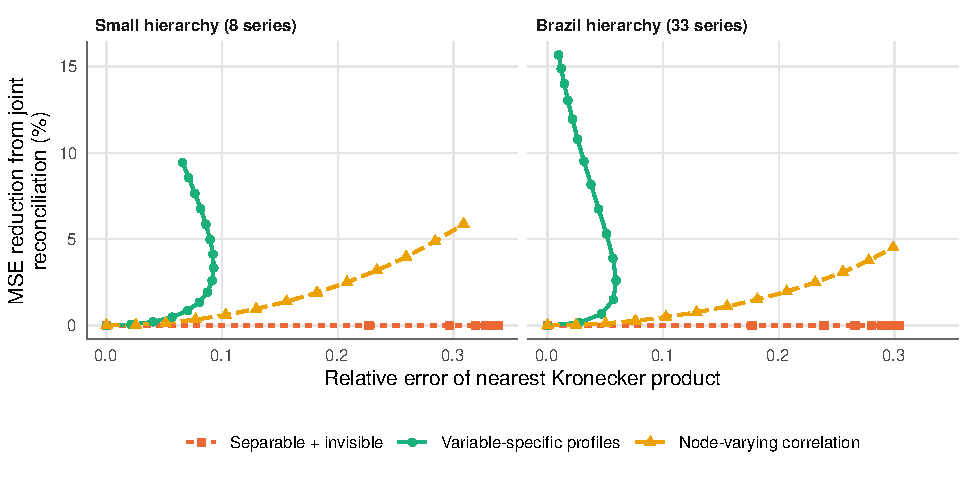
\includegraphics[width=\textwidth]{Imagens/kronecker_vs_gain.pdf}
  \caption{Population MSE reduction from joint reconciliation against the relative error of the nearest Kronecker approximation to $\bm{W}$, for the covariance families of Section~\ref{sec:simulation}.}
  \label{fig:kronecker}
\end{figure}

\subsection{Two measures}

We instead measure the conditions of Proposition~\ref{prop:equivalence} directly. The first measure describes the structure of the joint map. Since $\bm{G}$ contains the regression coefficients of the base forecast errors on the incoherences, and its off-diagonal blocks are the coefficients on other variables' incoherences, we define
\begin{equation}\label{eq:kappa}
  \kappa(\bm{W}) = \left(\frac{\sum_{j \ne k}\|\bm{G}_{jk}\|_F^2}{\|\bm{G}\|_F^2}\right)^{1/2},
\end{equation}
where $\bm{G}_{jk}$ is the $(n \times n_a)$ block of $\bm{G}$ relating the errors of variable $j$ to the incoherences of variable $k$. Rescaling variable $k$ by $c_k$ multiplies $\bm{G}_{jk}$ by $c_j/c_k$, so before computing $\kappa$ we standardise each variable by the square root of the mean diagonal of $\bm{W}_{jj}$. This makes $\kappa$ free of units. By Proposition~\ref{prop:equivalence}, $\kappa = 0$ exactly when joint and separate reconciliation coincide, and $\kappa$ inherits the invariance of Corollary~\ref{cor:invariance}.

The second measure describes the value of the joint map. If $\bm{W}$ were the true error covariance, the proportional reduction in mean squared error from reconciling jointly rather than separately would be
\begin{equation}\label{eq:gain}
  \gamma(\bm{W}) = 1 - \frac{\operatorname{tr}(\bm{M}\bm{W}\bm{M}')}{\operatorname{tr}(\bm{M}^{\mathrm{sep}}\bm{W}\bm{M}^{\mathrm{sep}\prime})}.
\end{equation}
MinT minimises the trace over all maps of this form, so $\gamma \ge 0$, again with equality exactly when the conditions of Proposition~\ref{prop:equivalence} hold. The two measures differ in an important way. The gain from any reconciliation comes only from the incoherent component of the errors, so $\gamma$ is small whenever that component is small, however strongly the joint map leans on other variables' incoherences. A large $\kappa$ with a small $\gamma$ says that joint reconciliation would change the forecasts but not improve them by much.

\subsection{Calibration}

Both measures are computed from an estimate $\widehat{\bm{W}}$, and both are biased in finite samples. Sampling noise pushes them above zero even when the population covariance satisfies Proposition~\ref{prop:equivalence}. The shrinkage estimator pulls the other way, because its diagonal target has no cross-variable blocks (Section~\ref{sec:theory}), so it shrinks genuine departures towards zero. Figure~\ref{fig:noise} shows both effects: \todo{describe noise floor and crossing, from exp1 results}. The raw values of $\kappa$ and $\gamma$ therefore cannot be read on an absolute scale.

\begin{figure}[!htb]
  \centering
  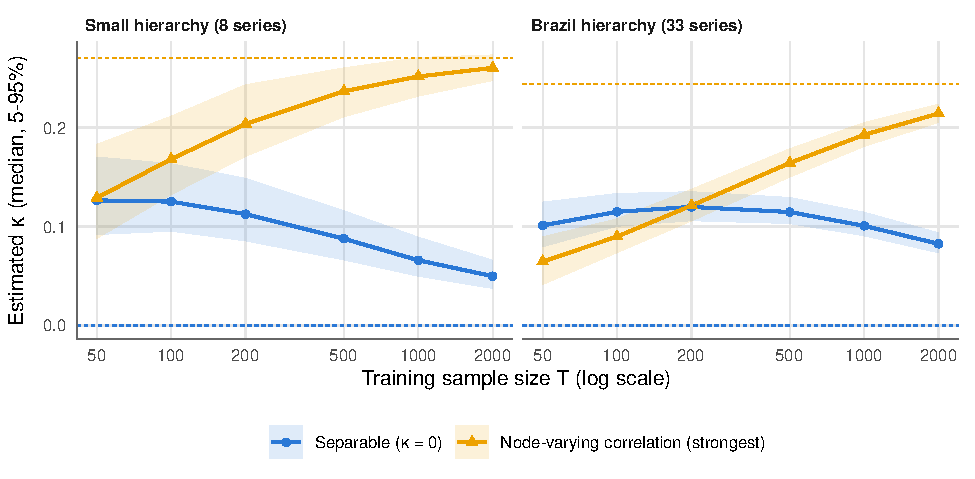
\includegraphics[width=\textwidth]{Imagens/kappa_noise.pdf}
  \caption{Sampling distribution of $\widehat\kappa$ (median and 5--95\% range over 1000 replications) under a separable covariance and under the strongest node-varying correlation case, with the population values dashed.}
  \label{fig:noise}
\end{figure}

We calibrate them with a parametric bootstrap that reproduces the estimation step:
\begin{enumerate}
  \item Estimate $\widehat{\bm{W}}$ from the $T$ residual vectors, and compute $\widehat\kappa$ and $\widehat\gamma$.
  \item Form the null covariance $\bm{W}_0$, the nearest Kronecker approximation to $\widehat{\bm{W}}$, which satisfies Proposition~\ref{prop:equivalence}.
  \item For $b = 1,\dots,B$, simulate $T$ vectors from $N(\bm{0}, \bm{W}_0)$, re-estimate the covariance with the same estimator, and compute $\kappa_b$ and $\gamma_b$.
  \item Report $p$-values $(1 + \#\{\kappa_b \ge \widehat\kappa\})/(B+1)$ and similarly for $\gamma$.
\end{enumerate}
The null covariance is one member of the set on which $\kappa = \gamma = 0$. It is the natural choice because it is the separable matrix closest to the data, but other members of the null set would give somewhat different null distributions. Figure~\ref{fig:power} reports the size and power of both tests for the covariance families of Section~\ref{sec:simulation}. \todo{summarise size and power, from power results}

\begin{figure}[!htb]
  \centering
  \includegraphics[width=\textwidth]{Imagens/gain_power.pdf}
  \caption{Rejection rate at the 5\% level of the bootstrap test based on $\widehat\gamma$ ($B = 199$, 200 replications), by sample size.}
  \label{fig:power}
\end{figure}

% Section 5 draft: simulations. Numbers are macros from Tabelas/numbers.tex.

\section{Simulations}
\label{sec:simulation}

We use two experiments. The first simulates base forecast errors directly, so that the population error covariance is known and the gain from joint reconciliation can be computed exactly. The second simulates time series, fits base forecasting models, and reconciles their forecasts, as in the original design of this study.

\subsection{Experiment 1: controlled error covariances}

For each of two variables, the base forecast errors are $\bm{e}_j = \bm{S}\bm{u}_j + \bm{v}_j$. The coherent component $\bm{S}\bm{u}_j$ is invisible to reconciliation (Corollary~\ref{cor:invariance}). The incoherent component $\bm{v}_j$ has independent entries across series, with variance $\lambda_{ij}$ for series $i$ and correlation $\rho_i$ between the two variables at series $i$. With this structure, condition (e) of Proposition~\ref{prop:equivalence} holds exactly when $d_i = \rho_i(\lambda_{i2}/\lambda_{i1})^{1/2}$ is the same for every series. We consider five families of covariance matrices, each indexed by a parameter that controls the departure from the conditions of Proposition~\ref{prop:equivalence}. Let $a_i$ be the number of bottom-level series summed by series $i$.
\begin{description}
  \item[F0, separable.] $\lambda_{i1} = \lambda_{i2} = a_i$ and $\rho_i = \rho$, with $\rho$ from $-0.9$ to $0.9$.
  \item[F1, separable plus invisible.] F0 with $\rho = 0.7$, plus a non-separable coherent component $\bm{S}_*\bm{K}\bm{S}_*'$ of increasing size.
  \item[F2, variable-specific profiles.] $\lambda_{i1} = a_i$, $\lambda_{i2} = a_i^{1+\delta}$ and $\rho_i = 0.7$. As $\delta$ grows, the second variable's incoherent errors become increasingly concentrated at the aggregate levels.
  \item[F3, node-varying correlation.] $\lambda_{i1} = \lambda_{i2} = a_i$ and $\rho_i = 0.3 + \delta z_i$, where $z_i \in [-1, 1]$ is a fixed pattern that alternates in sign within each level.
  \item[F4, OLS case.] $\bm{W} = \bm{S}_*\bm{K}\bm{S}_*' + \tau\bm{I}$.
\end{description}
F0, F1 and F4 satisfy Proposition~\ref{prop:equivalence}; F2 and F3 do not when $\delta > 0$. We use two hierarchies: the eight-series hierarchy of Figure~\ref{fig:HTS_M.ex}, and the 33-series hierarchy of the Brazilian application (Section~\ref{sec:application}).

\paragraph{Population results.} Figure~\ref{fig:exp1-gain} shows the exact MSE reduction from joint rather than separate reconciliation, $\gamma(\bm{W})$, against $\kappa(\bm{W})$. For F0, F1 and F4 both are zero to machine precision, whatever the strength of cross-variable correlation, and for F4 joint MinT coincides with OLS reconciliation. For F2 and F3 the gain rises with $\kappa$, but it is modest: at most \gainFtwoBrazilMax\% in the Brazilian hierarchy with $\kappa = \kappaFtwoBrazilMax$, and at most \gainFthreeSmallMax\% for node-varying correlations. Even substantial departures from the conditions of Proposition~\ref{prop:equivalence} buy little accuracy.

\begin{figure}[!htb]
  \centering
  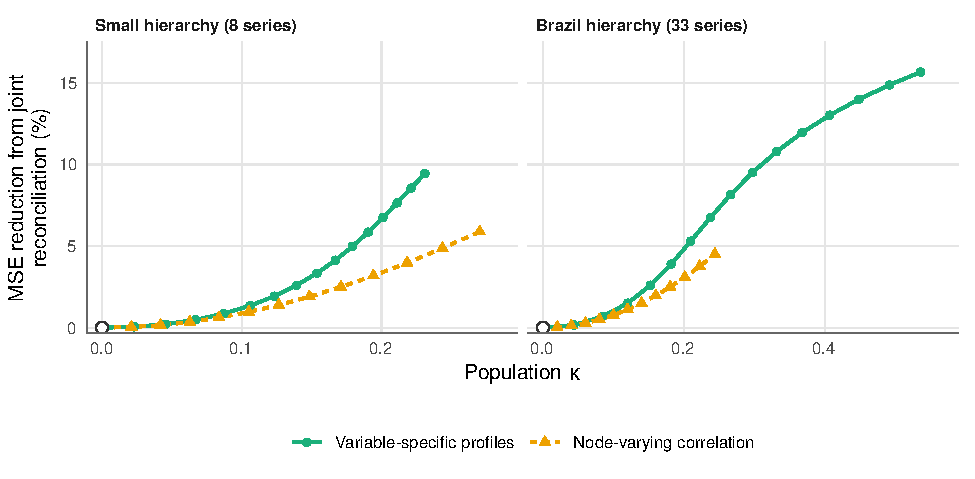
\includegraphics[width=\textwidth]{Imagens/exp1_gain.pdf}
  \caption{Experiment 1: population MSE reduction from joint rather than separate reconciliation against $\kappa$. The separable (F0), separable-plus-invisible (F1) and OLS (F4) families all lie at the origin.}
  \label{fig:exp1-gain}
\end{figure}

\paragraph{Estimated covariances.} In practice $\bm{W}$ is estimated, and the joint estimate has $m^2 = 4$ times as many entries as each separate one. For each family and hierarchy we drew $T \in \{50, 100, 200, 500, 1000, 2000\}$ error vectors from $N(\bm{0}, \bm{W})$, estimated the covariance by shrinkage \eqref{eq:shrink}, and computed the exact expected loss $\operatorname{tr}(\widehat{\bm{M}}\bm{W}\widehat{\bm{M}}')$ of the resulting maps, over \expOneReps{} replications. Figure~\ref{fig:exp1-T} shows the ratio of expected loss for joint to separate reconciliation. Under separability the joint map is never better, and it is worse at small sample sizes: by \sepPenaltySmall\% at $T = 50$ in the small hierarchy and \sepPenaltyBrazil\% in the Brazilian one. That is the price of estimating cross-variable blocks that carry no information. When the population gain is small, the estimated joint map does not recover it until $T$ is in the hundreds or thousands; for the weakest node-varying departure in the Brazilian hierarchy, whose population gain is \gainFthreeWeakBrazil\%, the estimated joint map gains only \gainFthreeWeakBrazilEst\% even at $T = 2000$. Only the largest departures give a clear gain at sample sizes typical of monthly data.

\begin{figure}[!htb]
  \centering
  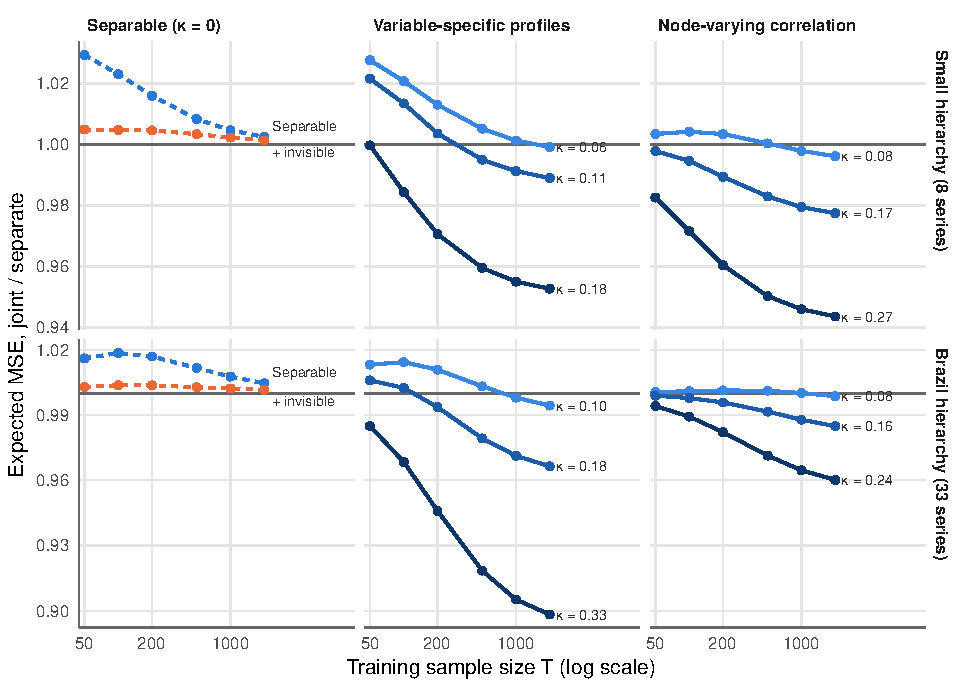
\includegraphics[width=\textwidth]{Imagens/exp1_samplesize.pdf}
  \caption{Experiment 1: expected MSE of joint relative to separate reconciliation with shrinkage estimates of $\bm{W}$, by training sample size. Values below one favour joint reconciliation. Labels give the population $\kappa$.}
  \label{fig:exp1-T}
\end{figure}

\subsection{Experiment 2: fitted base models}

\todo[inline]{Experiment 2: scenarios, population quantities (Table~\ref{tab:exp2}), fitted ARIMA and VAR results. Write after exp2 completes.}

\section{Application: admissions and dismissals in Brazil}
\label{sec:application}

\todo[inline]{Application.}

\section{Discussion}
\label{sec:discussion}

\todo[inline]{Discussion.}


\bibliographystyle{elsarticle-harv}
\bibliography{cas-refs}

\appendix
% Appendix draft: proofs for Section \ref{sec:theory}.

\section{Proofs}
\label{app:proofs}

\begin{proof}[Proof of Proposition~\ref{prop:equivalence}]
Let $\bm{Q} = \bm{C}_*\bm{W}\bm{C}_*'$, with blocks $\bm{Q}_{jk} = \bm{C}\bm{W}_{jk}\bm{C}'$. Because $\bm{W}$ is positive definite and $\bm{C}_*$ has full row rank, $\bm{Q}$ is invertible, so $\bm{G}$ is the unique solution of $\bm{G}\bm{Q} = \bm{W}\bm{C}_*'$. Block $(j,k)$ of the right-hand side is $\bm{W}_{jk}\bm{C}'$.

(c)$\Rightarrow$(a). Let $\bm{G} = \operatorname{diag}(\bm{H}_1, \dots, \bm{H}_m)$. Block $(j,j)$ of $\bm{G}\bm{Q} = \bm{W}\bm{C}_*'$ gives $\bm{H}_j\bm{C}\bm{W}_{jj}\bm{C}' = \bm{W}_{jj}\bm{C}'$, so $\bm{H}_j = \bm{G}_j$. Hence $\bm{M} = \bm{I} - \bm{G}\bm{C}_* = \operatorname{diag}(\bm{I} - \bm{G}_j\bm{C}) = \bm{M}^{\mathrm{sep}}$.

(a)$\Rightarrow$(b) is immediate.

(b)$\Rightarrow$(c). $\bm{G}\bm{C}_* = \bm{I} - \bm{M}$ is block diagonal. Since $\bm{C}_*$ is block diagonal with full row rank, it has the block diagonal right inverse $\bm{C}_*'(\bm{C}_*\bm{C}_*')^{-1}$, and $\bm{G} = (\bm{G}\bm{C}_*)\bm{C}_*'(\bm{C}_*\bm{C}_*')^{-1}$ is block diagonal.

(c)$\Leftrightarrow$(d). By the argument for (c)$\Rightarrow$(a), $\bm{G}$ is block diagonal if and only if $\bm{G} = \bm{G}^{\mathrm{sep}} = \operatorname{diag}(\bm{G}_1, \dots, \bm{G}_m)$. By uniqueness, this holds if and only if $\bm{G}^{\mathrm{sep}}\bm{Q} = \bm{W}\bm{C}_*'$. Blocks $(j,j)$ of this equation hold by the definition of $\bm{G}_j$. Blocks $(j,k)$ with $j \ne k$ read $\bm{G}_j\bm{C}\bm{W}_{jk}\bm{C}' = \bm{W}_{jk}\bm{C}'$, that is, $(\bm{I} - \bm{G}_j\bm{C})\bm{W}_{jk}\bm{C}' = \bm{M}_j\bm{W}_{jk}\bm{C}' = \bm{0}$. Finally, $\cov(\bm{M}_j\bm{e}_j, \bm{C}\bm{e}_k) = \bm{M}_j\bm{W}_{jk}\bm{C}'$.

(d)$\Leftrightarrow$(e). Condition (d) states $\bm{W}_{jk}\bm{C}' = \bm{W}_{jj}\bm{C}'\bm{B}_{jk}$ with $\bm{B}_{jk} = (\bm{C}\bm{W}_{jj}\bm{C}')^{-1}\bm{C}\bm{W}_{jk}\bm{C}'$, so (d) implies (e). Conversely, if $\bm{W}_{jk}\bm{C}' = \bm{W}_{jj}\bm{C}'\bm{B}$ for some $\bm{B}$, then $\bm{M}_j\bm{W}_{jk}\bm{C}' = \bm{M}_j\bm{W}_{jj}\bm{C}'\bm{B} = \bm{0}$, because $\bm{M}_j\bm{W}_{jj}\bm{C}' = \bm{W}_{jj}\bm{C}' - \bm{G}_j\bm{C}\bm{W}_{jj}\bm{C}' = \bm{0}$.
\end{proof}

\begin{proof}[Proof of Corollary~\ref{cor:invariance}]
Since $\bm{C}\bm{S} = \bm{0}$, we have $\bm{C}_*\bm{S}_* = \bm{0}$, so $(\bm{W} + \bm{S}_*\bm{K}\bm{S}_*')\bm{C}_*' = \bm{W}\bm{C}_*'$ and $\bm{C}_*(\bm{W} + \bm{S}_*\bm{K}\bm{S}_*')\bm{C}_*' = \bm{C}_*\bm{W}\bm{C}_*'$. Hence $\bm{G}$, and so $\bm{M}$, is unchanged. The diagonal blocks change by $\bm{S}\bm{K}_{jj}\bm{S}'$, which leaves each $\bm{G}_j$, and so $\bm{M}^{\mathrm{sep}}$, unchanged by the same argument.
\end{proof}

\begin{proof}[Proof of Corollary~\ref{cor:separable}]
Here $\bm{W}_{jk} = v_{jk}\bm{\Sigma}_0$, so $\bm{G}_j = \bm{\Sigma}_0\bm{C}'(\bm{C}\bm{\Sigma}_0\bm{C}')^{-1}$ and $\bm{M}_j = \bm{M}_0$ for every $j$. Then $\bm{W}_{jk}\bm{C}' = (v_{jk}/v_{jj})\bm{W}_{jj}\bm{C}'$, and condition (e) holds.
\end{proof}

\begin{proof}[Proof of Proposition~\ref{prop:coherent}]
Let $\bm{s}_a'$ be row $a$ of $\bm{S}$, and let $\bm{\Gamma}_h$ be the lag-$h$ autocovariance matrix of a VAR(1) with coefficient $\bm{\Phi}$ and innovation covariance $\bm{R}$. Since $\cov(\bm{\eta}_{i,t+h}, \bm{\eta}_{i',t}) = \sigma_{ii'}\bm{\Gamma}_h$, the stochastic component of series $(j,a)$, $\zeta_{j,a,t} = \sum_i s_{ai}\eta_{i,j,t}$, has autocovariances $\cov(\zeta_{j,a,t+h}, \zeta_{j,a,t}) = (\bm{s}_a'\bm{\Sigma}\bm{s}_a)[\bm{\Gamma}_h]_{jj}$. These are proportional across $a$, so the best linear predictor of $\zeta_{j,a,t+h}$ from $\zeta_{j,a,t}, \zeta_{j,a,t-1}, \dots$ applies the same linear filter $f_{j,h}$ at every node. A linear filter commutes with aggregation: $f_{j,h}(\zeta_{j,a,\cdot}) = \sum_i s_{ai} f_{j,h}(\eta_{i,j,\cdot})$. The deterministic components also aggregate, so the base forecasts of variable $j$ equal $\bm{S}$ times its bottom-level base forecasts and are coherent. The errors of coherent forecasts lie in the column space of $\bm{S}_*$, and any $\bm{S}_*\bm{P}$ with $\bm{P}\bm{S}_* = \bm{I}$ maps a vector $\bm{S}_*\bm{b}$ to itself.
\end{proof}


\end{document}
